\documentclass[11pt]{article}
\usepackage[margin=1in]{geometry}
\usepackage{times}
\usepackage[T1]{fontenc}
\usepackage{amsmath,amssymb}
\usepackage{graphicx}
\usepackage{booktabs}
\usepackage[numbers,sort&compress]{natbib}
\usepackage[hidelinks]{hyperref}
\usepackage{xcolor}
\usepackage{caption}
\captionsetup{font=small,labelfont=bf}
\graphicspath{{../figures/}}
\setlength{\parskip}{3pt}

\title{\textbf{Searching the Cognitive Possibility Space:}\\
A Computational Framework for Discovering Learnable Capabilities}
\author{Noam Shalom\\
\small Reichman University\\
\small \texttt{noamshalom77@gmail.com}}
\date{October 2026 \quad--- \quad working paper}

\begin{document}
\maketitle

\begin{abstract}
Reading is a capability evolution never selected for: culture found an input system that the
human brain can learn so well that it becomes automatic. This raises a question that is usually
not asked directly: \emph{what else could a fixed learner become, given the right interface and
training environment?} We formalise this as \textbf{Cognitive Capability Search (CCS)}: an outer
loop that searches over interfaces, objectives, input conditions and plasticity schedules for a
fixed-architecture learner, scored by how much new world structure becomes cheaply readable
(\emph{capability gain}) minus damage to existing abilities (\emph{interference}) --- without
naming a target capability. In a deliberately small toy (a modular neural network that
``develops'' with access to only half of its world's latent causes), CCS beats random search
under an equal budget in 10 of 10 worlds ($p=0.002$), and the environments it selects raise
few-shot performance on a held-out battery of tasks that depend on previously inaccessible
latents from $0.28$ to $0.51$--$0.60$ R$^2$. The search's most useful finding was one we did not
design in: \emph{acquire the new channel while the old sense is silent}. Changing only this one
setting moves interference from $\approx\!0.01$ to $0.35$--$0.97$; a revert test shows why ---
with the old sense silent, its pathway receives no gradient, so the search rediscovered gradient
isolation by choosing an input regime. Region-level ``adaptive plasticity'' did not beat global
plasticity, and the search exploited a gap in our first interference metric; closing the gap and
replicating in ten worlds left every finding standing. We report these as what a toy can show
--- a framing and a working method, not a claim about human brains.
\end{abstract}

\section{Motivation: reading as an existence proof}
Writing is roughly five thousand years old, far too recent for the brain to have evolved for it.
Yet literate adults read automatically, and reading is supported by a reproducible cortical
territory in the ventral visual stream. The \emph{neuronal recycling} hypothesis explains this by
saying that cultural inventions succeed when they fit pre-existing circuitry closely enough to
repurpose it \cite{dehaene2007}. Sensory substitution and augmentation make the same point from
the other side: tactile images can support visual-like perception \cite{bachyrita1969}, a
vibrating belt can become a usable sense of magnetic north \cite{nagel2005}, rats can learn to
perceive infrared light \cite{thomson2013} or navigate by a geomagnetic prosthesis
\cite{norimoto2015}, and skin can carry far more information than everyday life asks of it
\cite{novich2015}.

What these cases share is that \emph{someone guessed the capability first}, then built the
interface. Brain--machine interface research already treats the human and the decoder as two
co-adapting learners \cite{shenoy2014,perdikis2020}, but the task is still fixed in advance. This
paper asks a different question:
\begin{quote}
\emph{Can we systematically search for capabilities a learner is able to acquire, rather than
deciding the target capability in advance?}
\end{quote}
In other words, not ``how do I teach it $X$?'' but ``\emph{what can this learner become?}''

\section{Cognitive Capability Search}
\paragraph{Ingredients.} A learner $L$ with fixed architecture and partly developed weights; a
space $E$ of environments; and three measurements taken after $L$ is exposed to $e\in E$:
\begin{itemize}\itemsep0pt
\item \textbf{Capability gain} $G(e)$: how much more of the world's latent structure becomes
  \emph{cheaply} readable from $L$'s internal representation (few-shot linear probes
  \cite{alain2016}), relative to before.
\item \textbf{Interference} $I(e)$: loss of performance on abilities $L$ already had, read through
  their original, frozen readouts.
\item \textbf{Cost} $T(e)$: how long the learner had to be plastic.
\end{itemize}
CCS solves
\begin{equation}
e^\star=\arg\max_{e\in E}\; G(e)-\beta\, I(e)-\gamma\, T(e),
\end{equation}
with no term that names a particular capability. The probe bank is generic --- it asks about the
world's generative factors, not about a task we hope to see --- and a separate held-out task
battery, never used by the search, checks whether what was found is useful.

\paragraph{Two loops.} The \emph{inner loop} is ordinary learning: $L$ is trained on $e$'s
self-supervised objective. The \emph{outer loop} searches over $e$. Because the outer loop can
also choose \emph{which parts of $L$ are plastic and when}, a single environment can implement an
\emph{unlock $\to$ learn $\to$ select $\to$ consolidate} cycle, a computational analogue of
controlled critical periods \cite{hensch2005}.

\paragraph{Relation to existing work.} CCS borrows its machinery from open-ended search and
environment design (POET \cite{wang2019poet}, PAIRED \cite{dennis2020}, AI-generating algorithms
\cite{clune2019}), from novelty and quality-diversity search \cite{lehman2011,mouret2015}, from
intrinsic motivation \cite{oudeyer2007}, curriculum learning \cite{bengio2009} and meta-learning
\cite{hospedales2022}. The difference is the object of the search. Those methods mostly search for
environments that make an \emph{agent} better at a given objective, or generate ever-harder tasks.
CCS fixes the learner and asks which \emph{new capabilities} are reachable for it, and at what
price in interference with what it already does --- the stability--plasticity problem
\cite{mccloskey1989,kirkpatrick2017} as a constraint on the search space rather than as a nuisance.

\section{A toy instantiation}
\paragraph{World.} Eight latent causes $z\sim\mathcal N(0,I_8)$. The learner's innate sense
$s\in\mathbb R^{16}$ is a fixed nonlinear mixture of $z_0..z_3$ only; $z_4..z_7$ are invisible to
it.

\paragraph{Learner.} A small modular network (all code is pure NumPy):
$h_1=\tanh(W_1 s+b_1)$ (sensory region $R_1$), $h_c=\tanh(W_c c)$ (interface region $R_c$),
$h_2=\tanh(W_{2a}h_1+W_{2b}h_c+b_2+\eta)$ (association region $R_2$, intrinsic noise
$\eta\sim\mathcal N(0,0.2^2)$), and a readout $R_3$ predicting $z_0..z_3$. ``Development''
trains $R_1,R_2,R_3$ on the innate task with the new channel silent (innate R$^2=0.968$). The
pathway from $R_c$ into $R_2$ starts weak ($0.15\times$ normal scale), so at birth a new channel
reaches the association region only below the noise floor.

\paragraph{Environment space $E$.} Each environment is a genome:
\emph{interface} --- which latents a new 16-d channel carries (any subset of 8), its code
(\texttt{linear}, Gaussian-tuned \texttt{population}, high-frequency \texttt{phase}, or
\texttt{hashed} lookup) and noise level; \emph{objective} --- weights on reconstructing the channel
from $h_2$ and on \emph{aligning} channel-only $h_2$ to the representation the innate sense
produces (a direct ``recycling'' signal); \emph{input condition} during learning --- channel only,
both, or mixed; \emph{plasticity schedule} --- two phases, each unlocking any subset of
$\{R_1,R_c,R_2\}$ for $0$--$600$ steps; and learning rate --- about $1.5\times10^8$ distinct environments.

\paragraph{Measurements.} $G$ is the mean change in few-shot ($n{=}64$) ridge-probe R$^2$ for each
of the 8 latents from $h_2$, under two read-out conditions (channel only; sense + channel). $I$ is
the drop in innate-task R$^2$ through the frozen readout $R_3$, channel silent. $\beta{=}1$,
$\gamma{=}0.02$ per 1200 steps.

\paragraph{Outer loop and baselines.} A genetic algorithm (population 20, 12 generations,
tournament selection, crossover, mutation, 2 elites) gives 240 inner-loop runs per search. We
compare three plasticity regimes --- \emph{global} (all regions open for 600 steps), \emph{local}
(only $R_c$), and \emph{adaptive} (schedule searched) --- and random search over the adaptive space
with the same budget. Two hand-designed environments represent ``the obvious first guess'': carry
all latents in a clean linear code, train by reconstruction with both inputs present, under global
or local plasticity. Every result is repeated in three independently generated worlds (different
mixing, codes and learner initialisation); winners are re-tested with three fresh inner-loop seeds.
The full pipeline runs in about 15 minutes on two CPU cores.

\section{Results}

\begin{figure}[t]
\centering
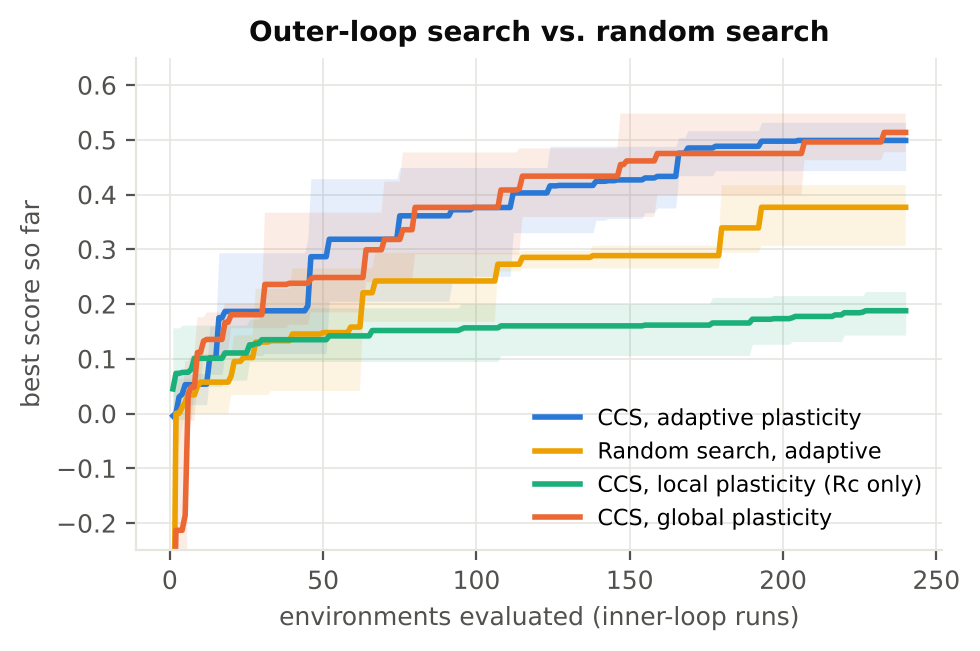
\includegraphics[width=0.49\linewidth]{fig1_search.png}\hfill
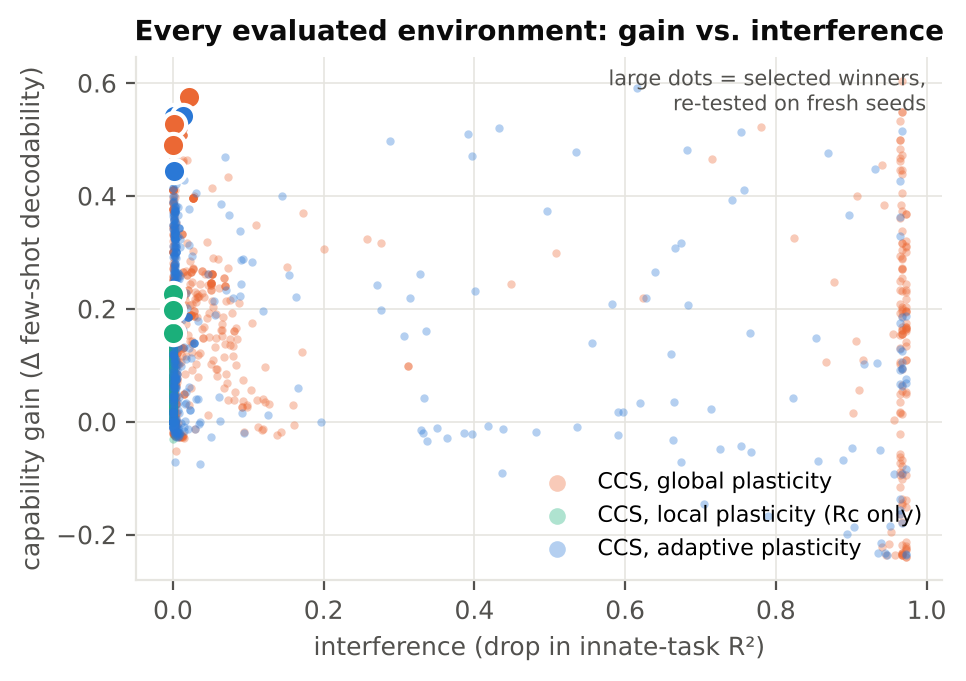
\includegraphics[width=0.49\linewidth]{fig2_tradeoff.png}
\caption{\textbf{Left:} best score found vs.\ number of inner-loop runs (mean over 3 worlds; band
= min--max). \textbf{Right:} every environment evaluated by the three CCS searches. Most of the
space trades capability for interference; the winners (large dots, re-tested on fresh seeds) sit
in the top-left corner.}
\label{fig:search}
\end{figure}

\paragraph{Search beats random sampling.} With 240 inner-loop runs, GA search reached a best
score of $0.50$ (adaptive) and $0.51$ (global) against $0.38$ for random search
(Fig.~\ref{fig:search}, left). Across 720 random environments only 3 ($0.4\%$) exceed $0.3$; the
GA crossed $0.3$ after 30--114 evaluations, random search after 137--192. Re-testing winners on
fresh seeds reproduced their scores (Table~\ref{tab:main}), so this is not a winner's-curse
artefact.

\paragraph{The capability that emerges.} Fig.~\ref{fig:profile} shows one selected environment.
Before exposure, the learner's association region carries essentially nothing about $z_4..z_7$.
After 150 steps in the selected environment, every carried latent is readable from the channel
alone (R$^2\approx0.92$), and with sense and channel together the hidden latents reach
R$^2\approx0.65$--$0.71$ while the visible ones stay at $0.90$--$0.93$. Across all three worlds,
the search consistently chose clean \texttt{linear} codes carrying 5--7 latents and avoided
\texttt{phase} and \texttt{hashed} codes, which on average \emph{reduced} decodability
(Fig.~\ref{fig:landscape}). That interfaces differ sharply in learnability is the toy analogue of
the recycling claim that only some cultural codes ``fit''.

\begin{figure}[t]
\centering
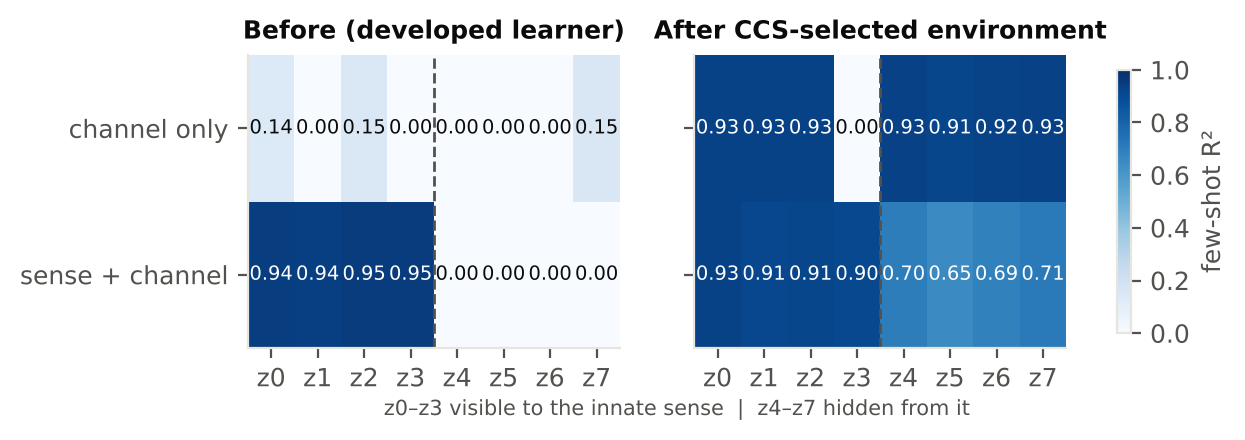
\includegraphics[width=0.92\linewidth]{fig3_profile.png}
\caption{Few-shot decodability of each latent from the association region, before and after the
CCS-selected environment (adaptive regime, world 0: carries $z_{0,1,2,4,5,6,7}$, linear code,
reconstruction objective, channel-only input, $R_c{+}R_2$ open for 150 steps).}
\label{fig:profile}
\end{figure}

\begin{table}[t]
\centering\small
\begin{tabular}{lcccccc}
\toprule
& \multicolumn{3}{c}{search objective (fresh seeds)} & \multicolumn{3}{c}{held-out battery, R$^2$}\\
\cmidrule(lr){2-4}\cmidrule(lr){5-7}
Condition & score & gain $G$ & interf.\ $I$ & all & visible & hidden\\
\midrule
No interface & --- & --- & --- & 0.379 & 0.829 & 0.283\\
Hand-designed, global & $-0.183$ & 0.661 & 0.834 & 0.740 & 0.785 & 0.730\\
Hand-designed, local & 0.121 & 0.131 & 0.000 & 0.460 & 0.819 & 0.384\\
Random search, adaptive & 0.378 & 0.390 & 0.002 & 0.514 & 0.796 & 0.454\\
CCS, global plasticity & \textbf{0.513} & 0.531 & 0.008 & 0.636 & 0.792 & 0.603\\
CCS, local plasticity & 0.184 & 0.194 & 0.000 & 0.403 & 0.825 & 0.314\\
CCS, adaptive plasticity & 0.499 & 0.509 & 0.005 & 0.620 & 0.795 & 0.583\\
\bottomrule
\end{tabular}
\caption{Means over 3 worlds $\times$ 3 inner-loop seeds. The battery is 40 random nonlinear
functions of 2--3 latents, read out few-shot from $h_2$ with sense and channel present; ``hidden''
tasks depend on at least one of $z_4..z_7$ (33 of 40).}
\label{tab:main}
\end{table}

\paragraph{Transfer to tasks the search never saw.} On the held-out battery
(Table~\ref{tab:main}, Fig.~\ref{fig:battery}), CCS-selected environments roughly double
performance on tasks that need a hidden latent ($0.28\to0.58$--$0.60$) at a small cost on tasks
over visible latents ($0.83\to0.79$). The hand-designed global environment does better still on
the battery ($0.73$) --- but it does so by destroying the learner's existing ability: innate-task
R$^2$ falls from $0.97$ to $0.11$. The battery fits fresh readouts and so cannot see this; the
interference term can. The two numbers have to be read together.

\begin{figure}[t]
\centering
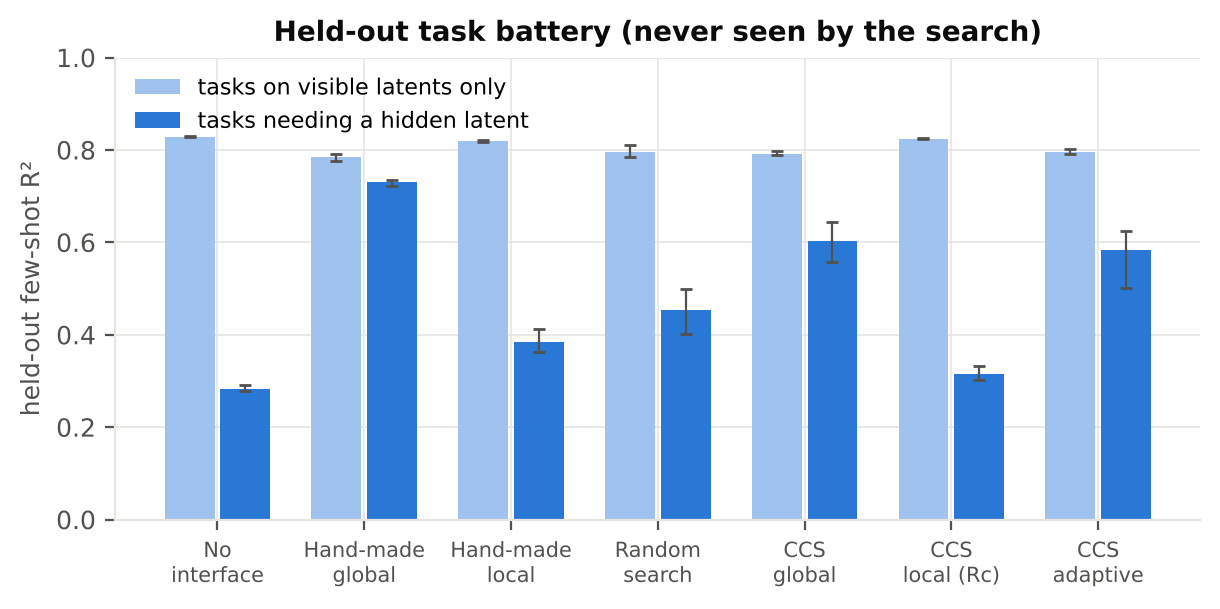
\includegraphics[width=0.78\linewidth]{fig4_battery.png}
\caption{Held-out battery, mean over 3 worlds (error bars = min--max).}
\label{fig:battery}
\end{figure}

\paragraph{What the search found that we did not design: learn while the old sense is silent.}
All twelve winners chose the \emph{channel-only} input condition. The CCS global winners differ
from the hand-designed global environment in small ways (one latent fewer, sometimes more noise or
a lower learning rate) and in one large way: they present the new channel \emph{without} the
innate sense. Table~\ref{tab:ablation} isolates this: holding everything else fixed and changing
only the input condition keeps the gain ($0.51$--$0.57$) but moves interference from $\le\!0.01$
to $0.35$--$0.97$.

\paragraph{Mechanism: input gating is gradient gating.} Two measurements explain it
(Table~\ref{tab:mech}). With $s=0$, the sensory weights $W_1$ receive exactly zero gradient and
$h_1$ is a constant vector, so the gradient on $W_{2a}$ is low-rank and its effect on real
sensory input is small: the input-dependent part of the change to $R_2$'s pre-activation is
$0.10$ signal-SD, against $0.79$ when the sense is present. A \emph{revert test} confirms where the
damage lives: after training with both inputs, restoring $W_1$ alone to its developed value
recovers $0.83$ of innate R$^2$ and restoring $W_{2a}$ recovers $0.44$; after channel-only
training there is nothing to recover. All adaptation went into the new pathway ($W_c$, $W_{2b}$).
In other words the search rediscovered \emph{gradient isolation} --- the principle behind weight
freezing, progressive networks and related continual-learning methods
\cite{kirkpatrick2017} --- by choosing an input regime, without being told anything about the
architecture, while the ``obvious'' hand-designed regime missed it. That is both the argument for
CCS and the limit of the claim: in hindsight the principle is familiar; what the search
contributes is finding it. The pattern is loosely reminiscent of the recruitment of deprived
cortex by Braille in blind readers \cite{sadato1996}, but we make no claim beyond the toy.

\begin{table}[t]
\centering\small
\begin{tabular}{lcccccc}
\toprule
& innate R$^2$ & \multicolumn{2}{c}{recovered by reverting} & \multicolumn{2}{c}{$\Delta$pre-activation (signal SD)} & $\|\Delta W_1\|/\|W_1\|$\\
\cmidrule(lr){3-4}\cmidrule(lr){5-6}
input during learning & after & $W_1$ & $W_{2a}$ & constant & input-dependent & \\
\midrule
channel only (as found) & 0.960 & 0.000 & 0.008 & 0.01 & 0.10 & 0.00\\
both & 0.068 & 0.827 & 0.443 & 0.02 & 0.79 & 0.23\\
\bottomrule
\end{tabular}
\caption{Mechanism of protection, CCS global winners, mean over 3 worlds. ``Recovered by
reverting'': gain in innate R$^2$ when that one parameter group is reset to its developed value
after acquisition. Reverting $b_1$, $b_2$, $W_c$ or $W_{2b}$ changes innate R$^2$ by $<0.001$ in
both conditions.}
\label{tab:mech}
\end{table}

\begin{table}[t]
\centering\small
\begin{tabular}{llccc}
\toprule
Winner & input during learning & gain & interference & score\\
\midrule
CCS, global & channel only (as found) & 0.531 & 0.008 & \textbf{0.513}\\
 & mixed & 0.571 & 0.968 & $-0.407$\\
 & both & 0.553 & 0.827 & $-0.284$\\
\midrule
CCS, adaptive & channel only (as found) & 0.509 & 0.005 & \textbf{0.499}\\
 & mixed & 0.546 & 0.763 & $-0.221$\\
 & both & 0.510 & 0.350 & 0.157\\
\bottomrule
\end{tabular}
\caption{Ablation: only the input condition is changed. Means over 3 worlds $\times$ 3 seeds.}
\label{tab:ablation}
\end{table}

\paragraph{Adaptive plasticity: a negative result, with a caveat.} We expected region-level
control (``open $R_2$ briefly, then freeze'') to beat global plasticity. It did not: $0.499$ vs.\
$0.513$ here, and $0.395$ vs.\ $0.409$ in the ten-world replication below ($p=0.75$). Once input gating was available, it did the work that
plasticity gating would otherwise do. The caveat is in Table~\ref{tab:ablation}: when the
protective input condition is removed, the adaptive winners' shorter, partial schedules keep
interference at $0.35$ against $0.83$ for global plasticity. Plasticity control looks like a second
line of defence rather than the main one --- suggestive only, with three worlds. Purely
\emph{local} plasticity (only the interface region) was the clearest failure: $R_c$ alone cannot
amplify a pathway into $R_2$ that starts below the noise floor, so gains plateaued at $\approx0.19$.
A new capability needed the association region to change.

\begin{figure}[t]
\centering
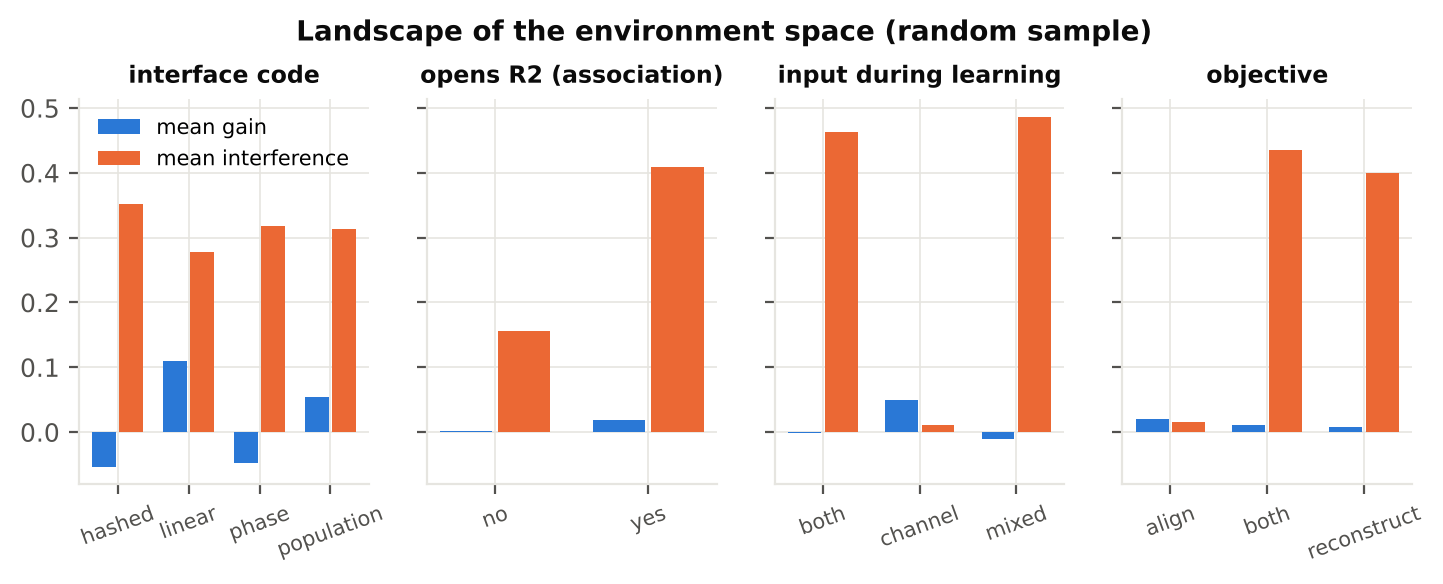
\includegraphics[width=\linewidth]{fig5_landscape.png}
\caption{Mean gain and interference per gene value, over 720 random environments (an unbiased
sample of $E$).}
\label{fig:landscape}
\end{figure}

\paragraph{The search exploited our metric.} Interference was measured with the new channel
silent. With the channel switched \emph{on}, CCS winners' innate-task R$^2$ drops from $0.97$ to
$0.88$ (vs.\ $0.31$ for the hand-designed global environment and $0.96$ for local plasticity).
Nothing in the score penalised this crosstalk, so the search did not avoid it. This is the general
lesson of any objective-driven search, and for CCS it is a design requirement: the interference
term must cover every context in which old abilities will be used.

\paragraph{Replication with the gap closed.} We therefore re-ran the study in ten independently
generated worlds with a corrected metric (``v2''): interference is the \emph{worse} of the innate
task's drop with the channel silent and with it on. Table~\ref{tab:robust} summarises; the
original three worlds are included. Every finding survives. CCS beats random search in all ten
worlds under the adaptive regime (sign test $p=0.002$) and nine of ten under the global regime
($p=0.021$), by $0.11$--$0.13$ score. Across the 2{,}400 random environments sampled in this run only
$0.3\%$ score above $0.3$; the adaptive search reaches $0.3$ in nine of ten worlds (median 99
evaluations), random search in four. All twenty winners again chose channel-only input and a
linear code, carrying 7 of the 8 latents on average. Adaptive and global plasticity remain
indistinguishable ($\Delta=-0.015\pm0.055$, adaptive better in 4 of 10 worlds). What the corrected
metric changed is informative in itself: the search did \emph{not} find an environment free of
crosstalk. The winners' innate R$^2$ with the channel on stays at $0.89$--$0.90$, so they now pay
the penalty (interference $0.07$--$0.08$, almost all of it crosstalk) for essentially the same
gain (on the same ten worlds, $0.47$--$0.50$ under v2 against $0.49$--$0.50$ under v1). Within
this environment space, some crosstalk appears to be the price of a new channel entering a shared
association region at all. Under the original metric on the same ten worlds the scores are
$0.488\pm0.042$ (global) and $0.476\pm0.043$ (adaptive), so the three-world numbers of
Table~\ref{tab:main} were not a lucky draw.

\begin{table}[t]
\centering\small
\begin{tabular}{lccccc}
\toprule
Condition & score (mean $\pm$ 95\% CI) & gain & interference & innate, channel on & battery, hidden\\
\midrule
Hand-designed, global & $-0.212\pm0.047$ & 0.658 & 0.860 & 0.295 & 0.726\\
Hand-designed, local & $0.111\pm0.014$ & 0.127 & 0.006 & 0.961 & 0.380\\
Random search, adaptive & $0.285\pm0.024$ & 0.357 & 0.065 & 0.903 & 0.401\\
CCS, global plasticity & $\mathbf{0.409\pm0.041}$ & 0.501 & 0.081 & 0.886 & 0.525\\
CCS, adaptive plasticity & $\mathbf{0.395\pm0.028}$ & 0.468 & 0.067 & 0.900 & 0.506\\
\bottomrule
\end{tabular}
\caption{Replication: 10 worlds, interference metric v2 (penalises crosstalk), winners re-tested
on 3 fresh seeds each. CI over worlds.}
\label{tab:robust}
\end{table}

\section{What this does and does not show}
It shows that, for a fixed learner, the space of interfaces and training regimes can be searched
\emph{for capabilities} rather than \emph{for a task}; that such search finds far better regions
of that space than random sampling; that what it finds transfers to tasks it never saw; and that
it can surface non-obvious training principles (here, input gating) that a designer can then test
directly. It also shows the method's main hazard: it optimises exactly the interference you
measure.

It does not show anything about human brains. The learner is a three-region $\tanh$ network; the
``capability'' is linear decodability of a synthetic world's factors; ten worlds and 240
evaluations per search are small, and the environment space is one we designed. The probe bank, though generic, is still a choice --- capabilities that are
not functions of $z$ (new kinds of computation rather than new information) are invisible to it.

\section{Why this might matter}
The near-term version of CCS is practical: searching the design space of sensory-substitution
devices, BCIs and training curricula with an explicit interference budget, using models of the
learner fitted to behavioural or neural data as the inner loop. The far version is a question:
are there cognitive modalities with no cultural analogue yet --- for example, a brain that has
learned to treat another person's neural state as an ordinary perceptual input --- sitting inside
the constraints of the human brain, undiscovered because nobody has built the right interface or
training environment? We do not claim this toy says anything about that. We claim it is the right
shape of question, and that it can be posed as a search.

\paragraph{Reproducibility.} Code, results and figures are released (NumPy and Matplotlib
only); \texttt{run\_experiments.py}, \texttt{run\_ablation.py}, \texttt{run\_mechanism.py} and
\texttt{make\_figures.py} regenerate every number here, and \texttt{--metric v2 --worlds 10}
reproduces the replication. Developed with AI assistance (Claude) for code and drafting.

\small
\bibliographystyle{unsrtnat}
\bibliography{refs}
\end{document}
